100. \begin{figure}[ht!]
\center{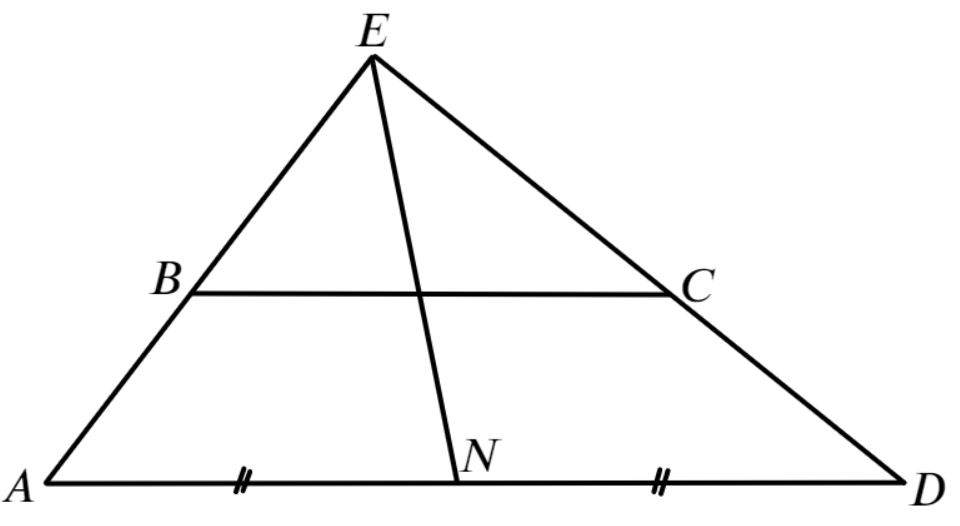
\includegraphics[scale=0.35]{g8-99.png}}
\end{figure}\\
Продлим боковые стороны трапеции до точки их пересечения $E.$ Тогда $\angle E=180^\circ-58^\circ-32^\circ=90^\circ.$ Пусть $N$ --- середина $AD,$ тогда $EN$ является медианой прямоугольного треугольника, проведённой из прямого угла, поэтому $EN=\cfrac{1}{2}AD=\cfrac{1}{2}\cdot22=11$см.\newpage\noindent
